\label{cha:analyse}
Für die Konzeption und Implementierung des Moodle-Plugins ist zunächst eine Analyse notwendig. Basierend auf einer Zielgruppenanalyse sollen Anforderungen an das Plugin bestimmt und priorisiert werden. Darauf aufbauend werden Möglichkeiten und Technologien zur Umsetzung des Hyperaudio-Plugins analysiert.

%\begin{figure}[h!]
%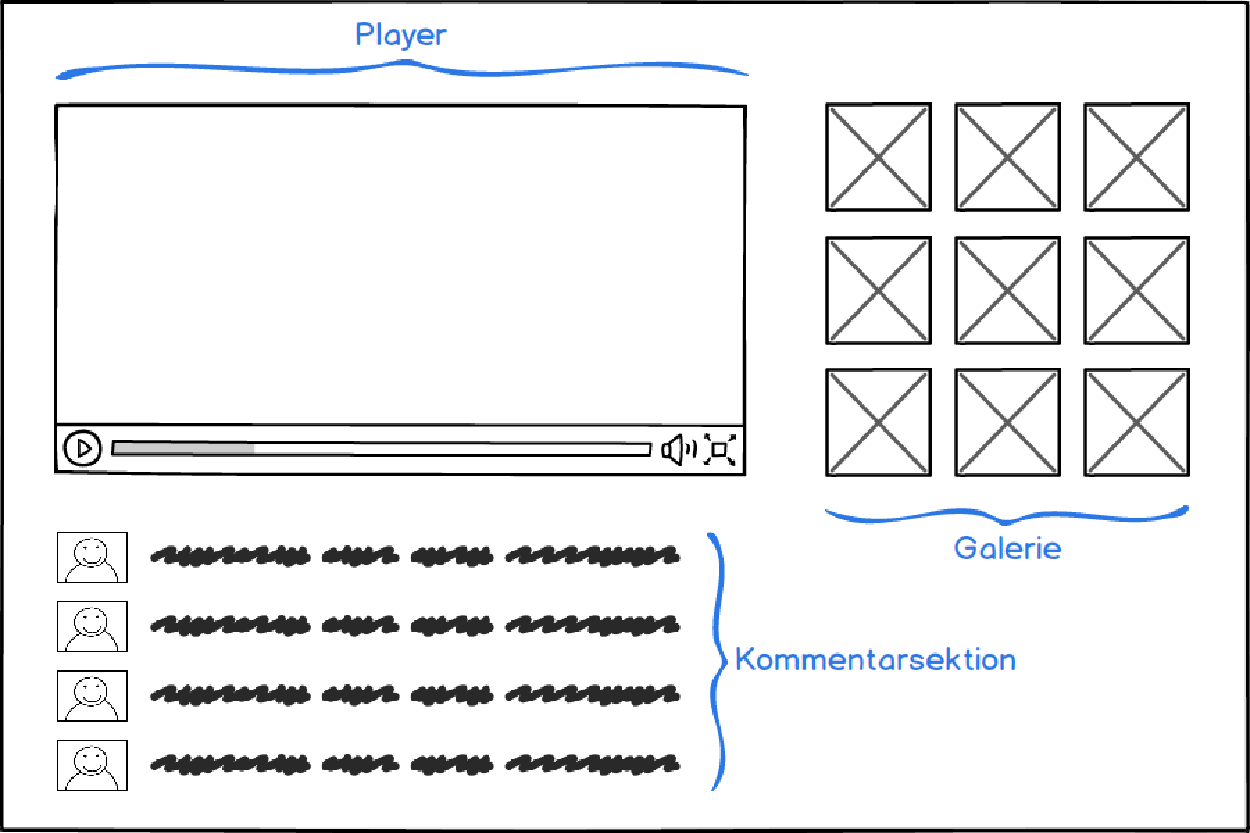
\includegraphics[width=.8\textwidth,center]{MockupBereiche.pdf}
%\caption{\label{fig:MockupBereiche}Erste Skizze der Moodle-Repräsentation eines Hyperaudio-Dokuments}
%\end{figure}


%%%%%%%%%%
\section{Zielgruppe}
Im ersten Schritt soll die Zielgruppe anhand von \textit{Personas} und deren \textit{User Stories} festgelegt werden. Dies soll dann die Grundlage für die Definition der Anforderungen im nächsten Abschnitt darstellen.


%%%%%%%%%%
\subsection{Personas}
\label{sec:personas}
%https://dl.gi.de/bitstream/handle/20.500.12116/5888/Holt_Winter_Thomaschewski_2011.pdf?sequence=2
Unter \textit{Personas} werden fiktive Benutzer verstanden, für welche das Programm, in unserem Fall das Moodle-Plugin, designt wird \citep{cooper2004inmates}. Jeder Persona wird eine Rolle im Zusammenhang mit der Anwendung zugewiesen. Darüber hinaus wird die Persona ausreichend beschrieben, damit sich leicht in die Person hineinversetzt werden kann \citep{cohn2004user}. Dieses Vorgehen hilft dabei, möglichst authentische \textit{User Stories} zu generieren, ohne auf echte Benutzer zurückgreifen zu müssen. Darüber hinaus ist festzustellen, dass die realen Anwender zwar Problemstellungen identifizieren können, aber nicht unbedingt in der Lage sind, Anforderungen zur Lösung dieser Probleme zu formulieren \citep{cooper2004inmates}. Für die Analyse und Konzeption des Hyperaudio-Plugins wird mit folgenden Personas gearbeitet:

\par
\begingroup
\leftskip=1cm
\rightskip=1.5cm
\noindent

{\Large\emph{Prof. Dr. Karolin Schröder}} ist verantwortlich für den Kurs \glqq Einführung in die Wirtschaftsinformatik\grqq{}. In diesem Kurs werden bereits erfolgreich Hyperaudio-Dokumente eingesetzt. Nachdem Prof. Dr. Schröder mit dem Start des nächsten Semesters überarbeitete Kurseinheiten anbietet, müssen nun auch die zugehörigen Hyperaudio-Dokumente auf die Notwendigkeit einer Überarbeitung hin überprüft werden. Die veralteten Hyperaudio-Dokumente müssen dann durch neuere Versionen ersetzt werden.
\vspace{.5cm}

{\Large\emph{Dr. Julian Schmidt}} ist wissenschaftlicher Mitarbeiter und Betreuer für den Kurs \glqq Marketing\grqq{}, der ebenfalls das Lernen mittels Hyperaudio-Dokument anbietet. Dr. Julian Schmidt ist unter anderem für die Betreuung dieser verantwortlich und ist derjenige, der hier Rede und Antwort steht.
\vspace{.5cm}

{\Large\emph{Laura Ebert}} ist 35 Jahre alt, verheiratet und hat drei Kinder. Sie geht halbtags ihrem Beruf als Anwendungsentwicklerin nach, zu dem sie 30 Minuten mit dem Bus pendelt. Neben der Arbeit kümmert sie sich zusammen mit ihrem Mann um den Haushalt und die Kinder. Laura studiert in Teilzeit den Bachelorstudiengang Informatik im ersten Semester. Das Semester hat erst vor einigen Wochen begonnen und sie entdeckt gerade Moodle für sich. Hierbei ist sie auf die Hyperaudio-Dokumente gestoßen und hat sich fest vorgenommen, sich im Laufe des Semsters mit deren Hilfe mit den Lerninhalten auseinanderzusetzen.
\vspace{.5cm}
 
{\Large\emph{Max Lustig}} ist 24 Jahre alt, ledig und hat sich nach einer abgeschlossenen Ausbildung zum Informatikkaufmann dazu entschlossen, neben dem Beruf zu studieren. Zur Arbeit kommt er in wenigen Minuten zu Fuß. Viel Zeit verbringt er jedoch im Fitnesstudio mit Kraft- und Ausdauertraining. Er absolviert ein Vollzeitbachelorstudium in Wirtschaftsinformatik und befindet sich kurz vor der Prüfungsphase zum Ende des dritten Semesters. Max möchte sich nun auf die Klausur des Moduls \glqq Investition und Finanzierung (BWL II)\grqq{}, welche in zwei Wochen stattfindet, intensiv vorbereiten. Im Laufe des Semsters hat er bereits ausgiebig die neuen Hyperaudio-Dokumente zum Erreichen des Lernziels genutzt.

\par
\endgroup

%%%%%%%%%%
\subsection{User Stories}
\label{sec:UserStories}
Unter Zuhilfenahme der entwickelten Personas werden im nächsten Schritt \textit{User Stories} formuliert. \textit{User Stories} beschreiben, wie die klassischen \textit{Use Cases}, Anforderungen an ein Softwaresystem. Diese sind dabei im Vergleich wesentlich oberflächlicher und ungenauer formuliert als \textit{Use Cases} \citep{wirdemann2017scrum}.

Erst im Laufe der Entwicklung werden \textit{User Stories} konkreter und dienen am Ende dazu, das Entwicklungsergebnis zu validieren. Beim Erstellen von \textit{User Stories} ist zu beachten, dass sogenannte \textit{Epics}, das sind \textit{User Stories} mit sehr großem Umfang, wenn möglich in kleinere \textit{User Stories} aufgesplittet werden. Unter anderem ist zu beachten, dass die \textit{User Stories} keine Abhängigkeiten untereinander aufweisen und dass deren Erfüllung überprüfbar ist. \textit{User Stories} können im \textit{Connextra Format} festgehalten werden, welches wie folgt aufgebaut ist \citep{cohn2004user}:

\par
\begingroup
\leftskip=1cm
\rightskip=1.5cm
\noindent

\textit{Ich als (Rolle) möchte (Funktion), um (Nutzen).}

\par
\endgroup

\vspace{.3cm}

Mit den Unterschieden und Einsatzzwecken von Personas und Rollen beschäftigt sich \cite{constantine2006users}. Grundsätzlich ist demnach festzustellen, dass Personas eher aus dem \textit{User-centered design} \citep{Norman1986user}, Benutzerrollen dagegen aus dem \textit{Usage-centered design} \citep{Constantine1996usage} motiviert sind. Während sowohl Personas als auch Benutzerrollen durchaus nützlich sind, um ein Verständnis von den Nutzern eines Systems zu erhalten, unterscheiden sie sich nach \cite{constantine2006users} in ihrer Philosophie und Relevanz für das Interaktionsdesign. Im Gegensatz zu Personas, die wie bereits im vorangegangenen Abschnitt \ref{sec:personas} beschrieben dazu dienen, die Nutzersicht anhand möglichst realer Personen darzustellen, sollen Benutzerrollen in einer wesentlich technischeren Sicht ein abstrahiertes Modell für die Art und Weise, in der Nutzer mit dem System interagieren, bilden \citep{constantine2006users}.

Für die weitere Analyse soll das Beste beider Welten vereinbart werden. Um die \textit{User Stories} möglichst anschaulich zu halten, werden sie anhand der vorgestellten Personas definiert. Gleichzeitig wird eine Aufteilung in Benutzerrollen vorgenommen, die die Grundlage für die Ableitung von Anforderungen aus den \textit{User Stories} bilden soll.

Für die Konzeption des Hyperaudio-Plugins ergeben sich im Wesentlichen zwei Benutzerrollen wie in Abbildung \ref{fig:Rollen} dargestellt. \textit{Administrierende} sind diejenigen Anwender, die Lerninhalte in Form von Hyperaudio-Dokumenten bereitstellen und verwalten. Diese Rolle kann nur von Lehrenden eingenommen werden. Die Gruppe der \textit{Nutzenden} kann derweil aus Lehrenden sowie Studierenden bestehen, die mit Hyperaudio-Dokumenten interagieren möchten.

\begin{figure}[h!]
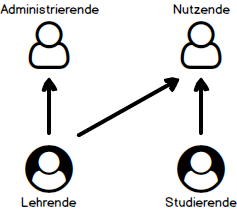
\includegraphics[width=.3\textwidth,center]{Rollen.png}
\caption{\label{fig:Rollen}Benutzerrollen}
\end{figure}


Für das Angebot einer Hyperaudio-Lernumgebung lassen sich folgende \textit{User Stories} festhalten:

\begin{enumerate}[label=US-\arabic*:,ref=US-\arabic*]

\item \label{US-Admin-Erstellen} Als Administrierende möchte Prof. Dr. Karolin Schröder ein neues Hyperaudio-Dokument in ihrem Kurs \glqq Einführung in die Wirtschaftsinformatik\grqq{} zur Verfügung stellen, um den Studierenden neue Lerninhalte bereitzustellen.

\item \label{US-Admin-Loeschen} Als Administrierende möchte Prof. Dr. Karolin Schröder Hyperaudio-Dokumente aus ihrem Kurs \glqq Einführung in die Wirtschaftsinformatik\grqq{} löschen können, um veraltete Informationen zu entfernen.

\item \label{US-Admin-Semester} Als Administrierende möchte Prof. Dr. Karolin Schröder Hyperaudio-Dokumente aus ihrem Kurs \glqq Einführung in die Wirtschaftsinformatik\grqq{} im Sommersemester in den darauffolgenden Kurs im Wintersemester übernehmen, um diese nicht erneut erstellen zu müssen.

\item \label{US-Admin-Kurs} Als Administrierende möchte Prof. Dr. Karolin Schröder Hyperaudio-Dokumente anderer Kurse in ihren Kurs \glqq Einführung in die Wirtschaftsinformatik\grqq{} übernehmen, um auf die hervorragende Arbeit anderer Lehrender zurückgreifen zu können, da sich die Themen mit ihrem Kurs überschneiden.

\item \label{US-Admin-Statistik} Als Administrierende möchte Prof. Dr. Karolin Schröder Erkenntnisse daraus gewinnen, wie die Hyperaudio-Dokumente des Kurses \glqq Einführung in die Wirtschaftsinformatik\grqq{} von Studierenden genutzt werden, um Verbesserungspotenzial auszumachen.

\item \label{US-Admin-Bearbeiten} Als Administrierender möchte Dr. Julian Schmidt ein vorhandenes Hyperaudio-Dokument in dem von ihm betreuten Kurs \glqq Marketing\grqq{} überarbeiten, um einen Fehler zu beseitigen.

\item \label{US-Wiedergabe} Als Nutzende möchte Prof. Dr. Karolin Schröder die bereits vorhandenen Hyperaudio-Dokumente aus ihrem Kurs \glqq Einführung in die Wirtschaftsinformatik\grqq{} wiedergeben, um diese auf ihre Richtigkeit zu überprüfen.

\item \label{US-Antwort-L} Als Nutzende möchte Prof. Dr. Karolin Schröder die Kommentare zu einem Hyperaudio-Dokument lesen und beantworten können, um auf Fragen von Studierenden einzugehen.

\item \label{US-Notiz-L} Als Nutzende möchte Prof. Dr. Karolin Schröder eine Notiz zu einem Hyperaudio-Dokument machen, um ihren Gedanken festzuhalten und später darauf zurückgreifen zu können.

\item \label{US-Kommentar-L} Als Nutzender möchte Dr. Julian Schmidt eine gefundene Erklärungslücke in einem Hyperaudio-Dokument durch einen Kommentar zum entsprechenden Zeitpunkt schließen, um eventuellen Fragen der Studierenden zuvorzukommen.

%\item \textit{Dr. Julian Schmidt stellt eine Erklärungslücke in einem Hyperaudio-Dokument fest und möchte diese durch einen Kommentar zum entsprechenden Zeitpunkt schließen.}

\item \label{US-Zeit} Als Nutzende möchte Laura Ebert mittels Hyperaudio-Dokument lernen, um die Zeit während Haushaltsarbeiten, wie dem Bügeln, Kochen oder Putzen, und dem Pendeln sinnvoller zu nutzen.

\item \label{US-Uebersicht-Kurse} Als Nutzende möchte Laura Ebert erfahren, welche Hyperaudio-Dokumente in den von ihr belegten Kursen angeboten werden, um herauszufinden, mit welchen Mitteln sie sich auf die anstehenden Prüfungen vorbereiten kann.

\item \label{US-Kommentar-S} Als Nutzende möchte Laura Ebert einen Kommentar verfassen, um dem Kursbetreuer und den anderen Studierenden eine Frage zu stellen.

\item \label{US-Markierung} Als Nutzende möchte Laura Ebert eine Markierung setzen, wenn eine klausurrelevante Thematik erklärt wird. Bei der Prüfungsvorbereitung möchte sie anhand dieser Markierungen diejenigen Themen erkennen, mit welchen sie sich besonders intensiv beschäftigen möchte.

\item \label{US-Markierung-Loeschen} Als Nutzende möchte Laura Ebert eine Markierung löschen, da sie den markierten Lerninhalt inzwischen beherrscht. Anhand der übrigen Markierungen möchte sie schnell erkennen, wo für sie noch Lernbedarf besteht.

\item \label{US-Notiz-S} Als Nutzende möchte Laura Ebert eine Notiz erstellen, um ein Beispiel zu dem genannten Sachverhalt festzuhalten, sodass sie die Thematik beim nächsten Mal einfacher nachvollziehen kann.

\item \label{US-Fortsetzen} Als Nutzende möchte Laura Ebert die Wiedergabe eines Hyperaudio-Dokuments beenden und am nächsten Tag automatisch an derselben Stelle fortsetzen können, um das Lernen schnell wiederaufnehmen zu können.

\item \label{US-Mobil} Als Nutzende möchte Laura Ebert die Hyperaudio-Angebote mit ihrem Smartphone in Anspruch nehmen, um auch die Zeit während des Pendelns zum Lernen nutzen zu können.

\item \label{US-Notiz-Bearbeiten} Als Nutzender möchte Max Lustig eine alte Notiz bearbeiten, um einen Schreibfehler zu korrigieren.

\item \label{US-Notiz-Loeschen} Als Nutzender möchte Max Lustig eine alte Notiz löschen, da er inzwischen Lernfortschritte gemacht hat und auf diese Notiz verzichten kann.

\item \label{US-Galerie} Als Nutzender möchte Max Lustig möchte schnell erkennen welche Inhalte im Hyperaudio-Dokument behandelt werden, um eine Erklärung eines bestimmten Themas zu finden.

\item \label{US-Suche} Als Nutzender möchte Max Lustig nach Textinhalten in Kommentaren suchen können, um schnell Erklärungen zu finden.

\item \label{US-Sortierung-Erstellungsdatum} Als Nutzender möchte Max Lustig die Kommentare nach Erstellungsdatum sortieren können, um sich einen Überblick über die neuesten Aktionen zu verschaffen.

\item \label{US-Sortierung-Zeitpunkt} Als Nutzender möchte Max Lustig die Kommentare und persönlichen Notizen zu den Annotationszeitpunkten zuordnen können, um diese bei der Wiedergabe verfolgen zu können.

\item \label{US-Filter} Als Nutzender möchte Max Lustig öffentliche Kommentare und persönliche Notizen getrennt betrachten können, um die öffentliche Diskussion verfolgen beziehungsweise die eigenen Anmerkungen isoliert betrachten zu können.

\item \label{US-Antwort-S} Als Nutzender möchte Max Lustig auf Kommentare antworten können, um sich mit den Studierenden und Lehrenden auszutauschen.

\item \label{US-Uebersicht-Letzte} Als Nutzender möchte Max Lustig erkennen, welche Hyperaudio-Dokumente er zuletzt abgespielt hat, um seinen Lernfortschritt im Auge zu behalten.

\item \label{US-Favoriten} Als Nutzender möchte Max Lustig besonders hilfreiche Hyperaudio-Dokumente als Favoriten speichern, um diese schnell als solche identifizieren zu können.

\item \label{US-Favoriten-Loeschen} Als Nutzender möchte Max Lustig die Markierung als Favorit entfernen können, wenn der Inhalt für ihn nicht mehr von Interesse ist.

\item \label{US-Zeit-Mobil} Als Nutzender möchte Max Ebert auf seinem Tablet Zugang zu Hyperaudio-Dokumenten haben, um die Zeit auf dem Laufband gleichzeitig zum Lernen nutzen zu können.

\end{enumerate}


%%%%%%%%%%
%\subsection{Umgebungsbedingungen}
%Aus den in Abschnitt \ref{sec:personas} beschriebenen \textit{Personas} und den in Abschnitt \ref{sec:UserStories} beschriebenen \textit{User Stories} können die Umgebungsbedingungen des \textit{Hyperaudio}-Plugins abgelesen werden. Diese stellen den Rahmen dar, in dem das Plugin durch die Studierenden genutzt werden können soll und spiegeln teilweise bereits Anforderungen wieder.
%
%So ergeben sich folgende Umgebungsbedingungen:
%
%\begin{itemize}
%\item Möglichkeit zur Nutzung des Plugins während der Ausübung anderer Tätigkeiten (Hausarbeit, Sport, Pendeln etc.)
%\item Unterstützung von verschiedenen Endgeräten (Desktop/Laptop, Tablet, Smartphone  etc.)
%\end{itemize}
%
%
%\todo[inline]{Rahmen in dem das Plugin durch Studierende genutzt werden können soll}
%- Während unbezahlter Arbeit
%- Beim Sport
%- An mobilen Endgeräten


%%%%%%%%%%
\section{Anforderungsdefinition}
\label{sec:anforderungsdefinition}
Basierend auf den \textit{Personas}, Rollen und \textit{User Stories} können nun die Anforderungen für das Hyperaudio-Plugin definiert werden. Hierbei werden aus einer oder mehreren \textit{User Stories} jeweils eine oder mehrere Anforderungen abgeleitet und zugleich mit einer Priorität versehen. Für die Priorisierung stehen die drei Prioritätsstufen \textit{niedrig}, \textit{mittel} und \textit{hoch} zur Verfügung. Bei der Priorisierung der Anforderungen soll die Zielsetzung aus Kapitel \ref{cha:einfuehrung} als Orientierung dienen.

%%%%%%%%%%
\subsection{Anforderungen der Administrierenden}
Es wird mit der Definition der Anforderungen der Administrierenden begonnen, welche in Tabelle \ref{tab:AnforderungenAdministrierenden} festgehalten werden. 

Aus \ref{US-Admin-Erstellen} kann die Anforderung des Erstellens von Hyperaudio-Dokumenten abgeleitet werden. Dass bestehende Hyperaudio-Dokumente auch bearbeitet und gelöscht werden können sollen, ergibt sich aus \ref{US-Admin-Bearbeiten} und \ref{US-Admin-Loeschen}. Zusammen stellen diese Anforderungen die Grundfunktionalitäten für die alternative Repräsentation der Lerninhalte dar und werden dementsprechend mit der Prioritätsstufe \textit{hoch} versehen.

Aus \ref{US-Admin-Semester} und \ref{US-Admin-Kurs} ergibt sich die Anforderung, dass Hyperaudio-Dokumente in einen anderen Kurs übernommen werden können sollen, sei es der gleiche Kurs im nächsten Semester oder ein anderer Kurs. Diese Anforderung zählt nicht zu den Grundfunktionalitäten, kann das Verwalten von Hyperaudio-Dokumenten jedoch vereinfachen und wird daher mit der Prioritätsstufe \textit{mittel} bewertet.

Der Wunsch, Erkenntnisse aus der Nutzung von Hyperaudio-Dokumenten durch die Studierenden zu erhalten (\ref{US-Admin-Statistik}), schlägt sich in der Anforderung nach statistischen Auswertungsmöglichkeiten nieder. Für diese Anforderung wird die Priorität \textit{niedrig} vergeben, da es sich um ergänzende Metainformationen handelt.

\begin{table}[!ht]
\def\arraystretch{1.4}
\caption{Anforderungen der Administrierenden}
\label{tab:AnforderungenAdministrierenden}
 \begin{tabularx}{\textwidth}{lXll}      
    \hline
    Nr. & Anforderung & Priorität
    \\\hline
    1 & Erstellen eines Hyperaudio-Dokuments & hoch\\
    2 & Bearbeiten eines Hyperaudio-Dokuments & hoch\\
    3 & Löschen eines Hyperaudio-Dokuments & hoch\\
    4 & Übernahme eines Hyperaudio-Dokuments in einen anderen Kurs & mittel\\
    5 & Statistische Auswertungen über die Nutzung der Hyperaudio-Dokumente & niedrig\\
    \hline
    \end{tabularx}
\end{table}


%%%%%%%%%%
\subsection{Anforderungen der Nutzenden}
Die aus den \textit{User Stories} der Nutzenden abgeleiteten Anforderungen sind in Tabelle \ref{tab:AnforderungenNutzenden} festgehalten. Die Priorisierung wird dabei nach folgenden Kriterien vorgenommen:

\begin{itemize}
\item \textit{hoch}: Basisfunktionalität zum Erreichen der Zielsetzung der Arbeit
\item \textit{mittel}: Verbesserung der Interaktion mit Hyperaudio-Dokumenten und Annotationen
\item \textit{niedrig}: Vereinfachter Zugriff auf Hyperaudio-Dokumente
\end{itemize}


Aus \ref{US-Wiedergabe}, \ref{US-Zeit}, \ref{US-Mobil} und \ref{US-Zeit-Mobil} ergibt sich die grundlegende Andorderung, Hyperaudio-Dokumente abspielen zu können. \ref{US-Zeit}, \ref{US-Mobil} und \ref{US-Zeit-Mobil} führen zudem zur Anforderung der Audio Cues, mithilfe derer auf annotierte Zusatzinhalte hingewiesen wird. Auch diese zählen neben der Wiedergabe zu den Basisfunktionalitäten, da erst dadurch das Ziel der größeren zeitlichen Flexibilität beim Lernen erreichbar wird (vgl. Abschnitte \ref{sec:zielsetzung} und \ref{sec:audiocues}). Um Inhalte schnell auffinden zu können, wie in \ref{US-Galerie} gefordert, ist eine Übersicht über annotierte Zusatzinhalte nützlich.

Basierend auf \ref{US-Antwort-L}, \ref{US-Kommentar-L}, \ref{US-Kommentar-S} \ref{US-Antwort-S} und \ref{US-Sortierung-Zeitpunkt} lässt sich die Anforderung an eine Kommentarfunktion ableiten, die über Möglichkeiten zum Erstellen, Anzeigen und Beantworten von Kommentaren verfügen muss. An dieser Stelle kann die Interaktion durch eine Suchfunktion innerhalb der Kommentare verbessert werden (vgl. \ref{US-Suche}). In den \textit{User Stories} \ref{US-Notiz-L}, \ref{US-Notiz-S}, \ref{US-Notiz-Bearbeiten}, \ref{US-Notiz-Loeschen} und \ref{US-Sortierung-Zeitpunkt} werden Wünsche bezüglich einer Notizfunktion formuliert. Diese lässt sich aufschlüsseln in die Anforderungen zum Erstellen, Anzeigen, Bearbeiten und Löschen von Notizen. Die Notizfunktion spiegelt das Ziel der Erhaltung typischer Nutzerinteraktionen mit textuellen Lernmedien wieder und kann das Lernen für die Studierenden erleichtern \citep{scutter2010students}. Ähnlich sind die Anforderung zum Erstellen, Anzeigen und Löschen von persönlichen Markierungen aus \ref{US-Markierung} und \ref{US-Markierung-Loeschen} zu bewerten. Obwohl Markierungen, ebenso wie die Notizfunktion, zu den Basisfunktionalitäten des Plugins gezählt werden können, wird die Markierungsfunktion mit der Priorität \textit{mittel} versehen. Das Herabsetzen der Priorität wird dadurch begründet, dass eine Markierung im Wesentlichen einer Notiz ohne textuellen Inhalt entspricht und durch die höher priorisierte Notizfunktion abgebildet werden kann. Aus \ref{US-Sortierung-Erstellungsdatum}, \ref{US-Sortierung-Zeitpunkt} und \ref{US-Filter} ergibt sich zudem der Wunsch nach Filter- und Sortiermöglichkeiten. 

Der Wunsch nach einer Favoritenfunktion für Hyperaudio-Dokumente ergibt sich aus \ref{US-Favoriten} und \ref{US-Favoriten-Loeschen}. Daraus resultieren die Anforderungen, Favoriten zu setzen, anzuzeigen und zu löschen. Übersichten über Hyperaudio-Dokumente werden in \ref{US-Uebersicht-Kurse} und \ref{US-Uebersicht-Letzte} gefordert: im ersten Fall eine Übersicht über alle Hyperaudio-Dokumente der belegten Kurse und im zweiten Fall eine Übersicht über die zuletzt abgespielten Hyperaudio-Dokumente. Sowohl die Favoritenfunktion als auch die Übersichten stellen eine reine Optimierung der Navigation dar und verhelfen somit zu einem vereinfachten Zugriff auf Hyperaudio-Dokumente. \ref{US-Fortsetzen} bringt die Anforderung für eine Funktion zum Fortsetzen unterbrochener Wiedergaben bei folgenden Aufrufen in Moodle hervor. Auch diese Funktion vereinfacht die Navigation zum gewünschten Hyperaudio-Dokument beziehungsweise dessen Inhalt.

Das Verlangen, Hyperaudio-Dokumente auch auf einem Smartphone oder Tablet nutzen zu können, wie in \ref{US-Mobil} und \ref{US-Zeit-Mobil} beschrieben, resultiert in der Anforderung zur Unterstützung von mobilen Endgeräten. Da es sich um eine Verbesserung der Interaktionsmöglichkeiten handelt, wird der Anforderung die Priorität \textit{mittel} zugewiesen.

\begin{table}[!ht]
\def\arraystretch{1.4}
\caption{Anforderungen der Nutzenden}
\label{tab:AnforderungenNutzenden}
\begin{tabularx}{\textwidth}{lXll}      
    \hline
    Nr. & Anforderung & Priorität
    \\\hline
    1 & Wiedergabe von Hyperaudio-Dokumenten & hoch\\
    2 & Hinweise auf die Darstellung von annotierten Zusatzinhalten & hoch\\
    3 & Übersicht über annotierte Zusatzinhalte & mittel\\
    4 & Kommentarfunktion bei Hyperaudio-Dokumenten & \\
    4.1 & \hspace*{0.5cm} Erstellen von Kommentaren & hoch\\
    4.2 & \hspace*{0.5cm} Anzeigen von Kommentaren & hoch\\
    4.3 & \hspace*{0.5cm} Antworten auf Kommentare & hoch\\
    4.4 & \hspace*{0.5cm} Suchfunktion innerhalb der Kommentare & mittel\\ 
    5 & Notizfunktion bei Hyperaudio-Dokumenten & \\
    5.1 & \hspace*{0.5cm} Erstellen von Notizen & hoch\\
    5.2 & \hspace*{0.5cm} Anzeigen von Notizen & hoch\\
    5.3 & \hspace*{0.5cm} Bearbeiten von Notizen & hoch\\
   	5.4 & \hspace*{0.5cm} Löschen von Notizen & hoch\\
    6 & Markierungsfunktion bei Hyperaudio-Dokumenten & \\
    6.1 & \hspace*{0.5cm} Erstellen von Markierungen & mittel\\
    6.2 & \hspace*{0.5cm} Anzeigen von Markierungen & mittel\\
   	6.3 & \hspace*{0.5cm} Löschen von Markierungen & mittel\\
   	7 & Filter- und Sortiermöglichkeiten & mittel\\
    8 & Favoritenfunktion für Hyperaudio-Dokumente & \\
    8.1 & \hspace*{0.5cm} Erstellen von Favoriten & niedrig\\
    8.2 & \hspace*{0.5cm} Anzeigen von Favoriten & niedrig\\
    8.3 & \hspace*{0.5cm} Löschen von Favoriten & niedrig\\    
    9 & Übersicht über alle Hyperaudio-Dokumente der belegten Kurse & niedrig\\
    10 & Übersicht über die zuletzt abgespielten Hyperaudio-Dokumente & niedrig\\
    11 &  Funktion zum Fortsetzen unterbrochener Wiedergaben bei folgenden Aufrufen in Moodle & niedrig\\
    12 & Unterstützung von mobilen Endgeräten & mittel\\
    \hline
\end{tabularx}
\end{table}

%%%%%%%%%%
\section{Möglichkeiten der Moodle Plugin-Entwicklung}
Für den Betrieb von Moodle werden ein Webserver, eine MySQL- oder PostgreSQL-Datenbank und PHP vorausgesetzt \Citep{moodle2018install}. Moodle unterstützt die Verwendung von JavaScript und die Einbindung von Thirdparty-Frameworks \citep{wild2017moodle}. Dies gepaart mit den Möglichkeiten durch den Einsatz von PHP bietet bei der Entwicklung ausreichend Möglichkeiten um das gewünschte Plugin umzusetzen.

Des Weiteren wird die Entwicklung von Moodle mithilfe der sogenannten \textit{Core APIs} (Application Programming Interface) unterstützt.
\todo[inline]{APIs ergänzen}

\textbf{Zu Beginn der Entwicklung eines Moodle-Plugins steht jedoch die Frage, um welche Art von Plugin es sich handelt.} Es werden nun diejenigen Plugin-Typen beschrieben, welche für das Hyperaudio-Plugin infrage kommen \citep{moodle2017plugin}.


\subsubsection{Media Player}
Mit diesem Plugin-Typ kann Moodle um alternative Player für Audio- und Videoformate, aber auch für andere Medien (z.B. Diagramme, Formeln, etc.) ergänzt werden \citep{moodle2017media}. Player beziehen sich aber stets auf das reine Abspielen von Dateien oder Links zu externen Medieninhalten, wie zum Beispiel ein Link zu einem \textit{Youtube}-Video.

%Media players are used to automatically embed files in the pages. It is normally video or audio files or links to media sharing sites such as YouTube or Vimeo. However it is also possible to use media players for embedding other contents - diagrams, formulas, etc. Media players usually look at the file extension to match with the player but they can also make a URL match (this can be used for YouTube, Vimeo and similar sites links).

\subsubsection{Blöcke}
Blöcke dienen dazu, Kursseiten um zusätzliche Informationen anzureichern, welche dann in der rechten oder linken Spalte angeheftet werden können (siehe Abbildung \ref{fig:MoodleKursseitenbeispiel}). Blöcke können auch \glqq angeheftet\grqq{} werden \citep{moodle2018blocks}. Diese Anheftung kann auf verschiedene Bereiche erfolgen, beispielsweise in der gesamten Moodle-Umgebung, auf der Seite des Benutzerprofils oder der Startseite \citep{moodle2015blocksettings}. Blöcke sind also nicht dazu geeignet größere Inhalte darzustellen. Dementsprechend kommt dieser Plugin-Typ nicht für unser Hyperaudio-Plugin in Frage. Es wäre aber durchaus denkbar, dass mithilfe von Blöcken die Anforderungen 8.2, 9 und 10 umgesetzt werden könnten.  


\subsubsection{Ressourcen}
Mittels eines Plugins dieses Typs ist es möglich, dem Studierenden Inhalte zu präsentieren, wobei dieses Plugin keinerlei Eingabe oder Interaktion von Seiten des Studierenden erwartet und ausschließlich dazu dient, Informationen darzustellen \citep{wild2017moodle}.
%A Moodle resource plugin transmits information to the learner--it expects nothing in return.
%A resource plugin expects the learner to be passive. Obvious examples of resources are text
%to read, videos to watch, and audio to listen to. That is not to say that the resource won't
%form the basis of some form of interaction outside of Moodle, but we certainly don't expect
%any aspect of that interaction to be captured in Moodle


\subsubsection{Aktivitäten}
Neben der Darstellung von Inhalten erwarten Aktivitäten im Gegensatz zu Ressourcen eine Art von Interaktion durch den Studierenden. Dies kann beispielsweise in Form eines Quiz, bei dem der Nutzer Antworten anhaken muss, oder in Form eines Forums, in dem der Studierende Beiträge schreibt, geschehen \citep{wild2017moodle}. Aufgrund des interaktiven Charakters stellen Aktivitäten den richtigen Plugin-Typ für das Hyperaudio-Plugin dar.
%Compared to a resource, an activity expects some form of learner interaction - this is
%Moodle in receive mode. This could be an obvious example, such as a quiz where the
%learner will type in a response for Moodle to mark, or it could be a forum where social
%constructionist learning takes place.


%%%%%%%%%%
\section{Aktueller Stand der Technik}
\textbf{Es wird zunächst der aktuelle Stand der Technik bezüglich der Zielsetzung dieser Arbeit betrachtet.} Hierbei werden im ersten Schritt bereits etablierte Plattformen für die Bereitstellung von Audio- und Videoinhalten begutachtet. Im zweiten Schritt werden dann vorhandene Technologien für die Umsetzung innerhalb von Moodle untersucht.


%%%%%%%%%%
\subsection{Etablierte Audio- und Video-Plattformen}

Mit dem Hintergrund, eine nach DIN EN ISO 9241 erwartungskonforme Software gestalten zu wollen, erfolgt nun zunächst eine Analyse von etablierten Systemen zur Wiedergabe von Audio- und Videoinhalten mit integrierten Kommunikationsmöglichkeiten. Da menschliches Handeln stark durch erlernte Verhaltensmuster geprägt ist, empfiehlt es sich, bei der Gestaltung von Interaktionen auf bekannte Verfahren zurückzugreifen, um den kognitiven Aufwand zum Erlernen der Bedienmöglichkeiten gering zu halten und somit eine Konzentration auf die wesentlichen Inhalte zu ermöglichen \citep{erwartungskonformitaet}.

%\todo[inline]{ Unpassende Einleitung, oder? Beschreiben Sie ruhig ein bisschen mehr. Z.B. die Kommentarfunktion.}

\subsubsection{SoundCloud}

\glqq Als weltweit größte Musik- und Audio-Plattform\grqq{} \citep{soundcloudinfo} bietet \textit{SoundCloud} Künstlern eine Plattform, um ihre Musik einem breiten Publikum anzubieten. Charakteristisch für \textit{SoundCloud} ist das Design des Players (siehe Abbildung \ref{fig:SoundCloudPlayer}). Zum einen wird hier die Waveform des Musikstückes angezeigt und zum anderen werden gleichzeitig mittels Thumbnails Kommentare an ebenjener Stelle des Stücks visualisiert, zu der kommentiert wurde. Beim Abspielen des Musikstücks werden die annotierten Kommentare zum jeweiligen Zeitpunkt eingeblendet. Zusätzlich bietet der Player auch durch Mouseover-Effekte auf den Thumbnails die Möglichkeit, die annotierten Kommentare zu lesen. Durch einen Klick auf das entsprechende Thumbnail kann direkt auf den Kommentar geantwortet werden. Unterhalb des Players befindet sich der Eingabebereich, um eigene Kommentare zu verfassen. Diese werden zu dem Zeitpunkt gespeichert, zu dem der Kommentar begonnen wurde. Wiederum unterhalb des Eingabebereichs befindet sich ein Bereich für die Anzeige der Kommentare. Sie werden chronologisch nach Erstellungsdatum, mit dem neusten Kommentar an oberster Stelle, dargestellt. Antworten auf Kommentare werden durch eine leichte Einrückung gekennzeichnet.

\begin{figure}[h!]
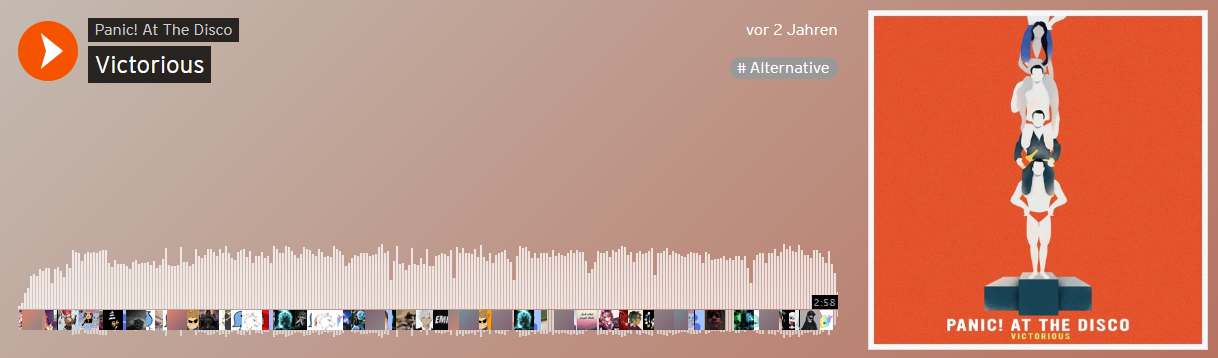
\includegraphics[width=.9\textwidth,center]{SoundCloudPlayer.png}
\caption{\label{fig:SoundCloudPlayer}Player der Musik- und Audio-Plattform \textit{SoundCloud} \citep{SoundCloud2015Panic}}
\end{figure}

\subsubsection{Youtube}
 
Im Bereich der Videoplattformen gilt \textit{Youtube} als die mit Abstand am weitesten verbreitete Videoplattform in Deutschland \citep{statista2016video}.  Zum Abspielen der von den Nutzern hochgeladenen Videos setzt \textit{Youtube} auf den HTML5-Player\footnote{HTML = HyperText Markup Language} (siehe Abbildung \ref{fig:YoutubePlayer1}).

\begin{figure}[h!]
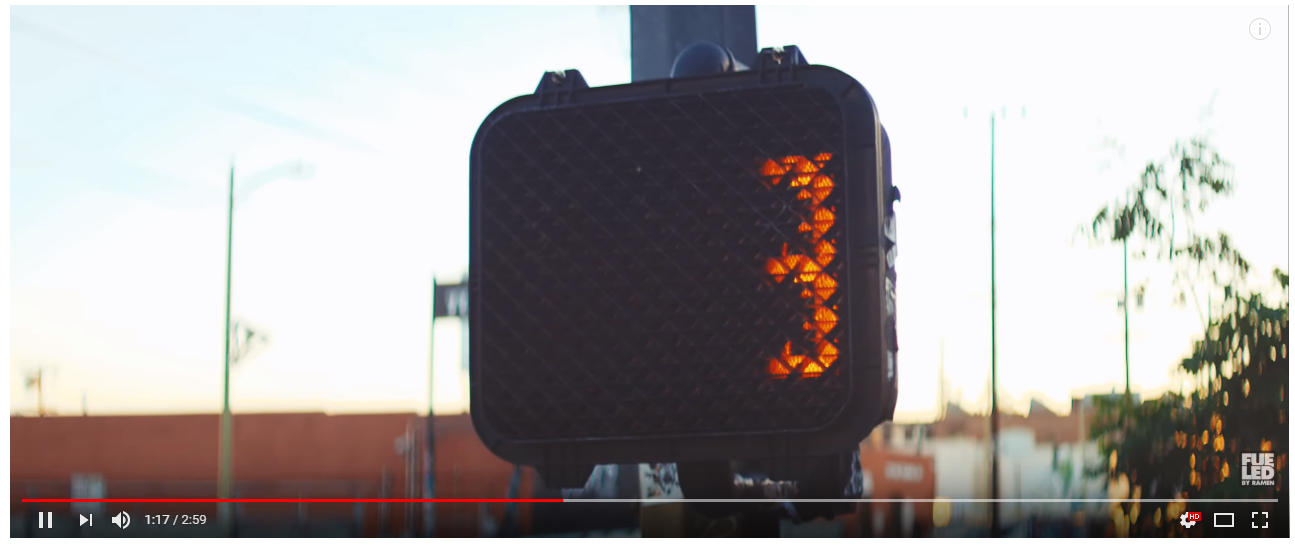
\includegraphics[width=.9\textwidth,center]{YoutubePlayer1.png}
\caption{\label{fig:YoutubePlayer1}Player der Video-Plattform \textit{Youtube} \citep{Youtube2015Panic}}
\end{figure}

In \citep{youtubeinfokarten,youtubeabspann} werden Möglichkeiten aufgezeigt, Informationen an ein Video zu annotieren. Die Informationen können Verweise auf andere Videos, Playlists und Kanäle, eine Abstimmung oder einen Link zu einer Webseite beinhalten. Einem Video können insgesamt maximal ein Abspann und bis zu fünf Infokarten mittels des integrierten Webeditors angeheftet werden. Bei Infokarten kann nur der jeweilige Startzeitpunkt für die Anzeige frei festgelegt werden, die Dauer wird durch \textit{Youtube} vorgegeben. Abbildung \ref{fig:YoutubePlayer2} zeigt, wie eine solche Infokarte im Player dargestellt wird. Ein Abspann kann hingegen nur während der letzten fünf bis 20 Sekunden eines Videos angezeigt werden.

\begin{figure}[h!]
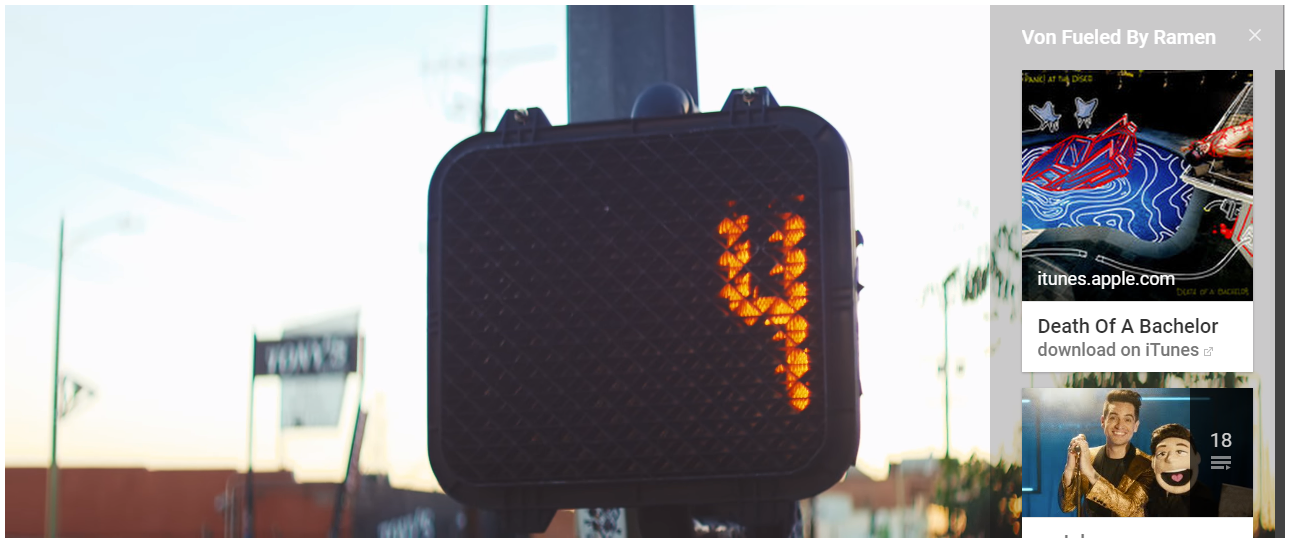
\includegraphics[width=.9\textwidth,center]{YoutubePlayer2.png}
\caption{\label{fig:YoutubePlayer2}Anzeige der Infokarte \citep{Youtube2015Panic}}
\end{figure}


%%%%%%%%%%
\subsection{Technologien für den Einsatz in Moodle}
Bevor mit der Konzeption und Implementierung des Moodle-Plugins begonnen wird, wird sich nun der Analyse bestehender Komponenten zugewendet, die als Basis für das Plugin dienen könnten. Ziel ist es festzustellen, ob bereits Technologien existieren, mit deren Hilfe die Idee des Hyperaudio-Plugins umgesetzt werden kann oder ob zumindest Teile davon - unter entsprechender Beachtung der Lizenzierung - sinnvoll wiederverwendet werden können. \textbf{Hierbei wird so vorgegangen, dass die einzelnen vorhanden Technologien auf diesem Gebiet und ihre Funktionen vorgestellt und anschließend bewertet werden, inwiefern diese für die Umsetzung des Plugins relevant sind.}

%%%%%%%%%%
\subsubsection{VideoJS Player}
Bei dem \textit{VideoJS Player}\footnote{GitHub-Projekt, Apache-Lizenz 2.0: http://videojs.com/; https://github.com/videojs} handelt es sich um eine Open-Source-Bibliothek zum Abspielen von Videos und stellt damit einen HTML5-Video-Player zur Verfügung. Der \textit{VideoJS Player} ist bereits als Standard-Plugin für die Wiedergabe von Audio- und Video-Dateien in Moodle integriert. Wie der Name schon erkennen lässt, handelt es sich hierbei um eine JavaSrcipt-Bibliothek. Der \textit{VideoJS Player} beschränkt sich in seiner Ausgangsversion ausschließlich auf das Abspielen von Audio- und Video-Dateien und bietet bis auf ein optionales Fallback auf den Adobe FlashPlayer keine weiteren Funktionen. Die Funktionalität des \textit{VideoJS Player} kann aber über Plugins erweitert werden. Es existieren bereits zahlreiche solcher Plugins. Hier sei vor allem das Plugin \textit{videojs-wavesurfer}\footnote{GitHub-Projekt, MIT Lizenz: https://github.com/collab-project/videojs-wavesurfer} genannt, welches das \textit{wavesurfer.js}-Framework (siehe Abschnitt \ref{sec:wavesurfer.js}) in den \textit{VideoJS Player} integriert. Dank der Unterstützung von Plugins ist es durchaus denkbar, den Player mittels Plugin beispielsweise um Buttons zum Erstellen von Kommentaren oder persönlichen Notizen zu erweitern. Auch wäre es denkbar, mittels eines Plugins die annotierten Kommentare zu visualisieren. Grundsätzlich stellt der \textit{VideoJS Player} somit eine gute Ausgangslage für einen Hyperaudio-Player dar.

%%%%%%%%%%
\subsubsection{H5P}
Mit \textit{H5P} und dem bereits vorhanden Plugin für Moodle\footnote{GitHub-Projekt, GNU General Public License v2.0: https://github.com/h5p/h5p-moodle-plugin} ist es möglich, verschiedene Arten von interaktiven Lerninhalten zu gestalten. Dabei handelt es sich um eine Sammlung von interaktiven Komponenten, darunter \textit{Course Presentation}, \textit{Timeline} und \textit{Interactive Video}. \textit{Course Presentation} bietet die Möglichkeit, interaktive Präsentationen zu gestalten. \textit{Timeline} kann genutzt werden um Inhalte anhand eines Zeitstrahls darzustellen. \textit{Interactive Video} ermöglicht, ähnlich wie \textit{Course Presentation}, die Interaktion während des Abspielens eines Videos (siehe Abbildung \ref{fig:H5P}). Besonders erwähnenswert ist, dass sich die interaktiven Inhalte bei \textit{H5P} innerhalb der Weboberfläche erstellen lassen. Es wäre also denkbar, eine eigene interaktive Komponente zu entwickeln, welche es ermöglicht, Hyperaudio-Dokumente als interaktiven Lerninhalt zu erstellen und abzuspielen sowie eine Kommentarfunktion zu integrieren.

\begin{figure}[h!]
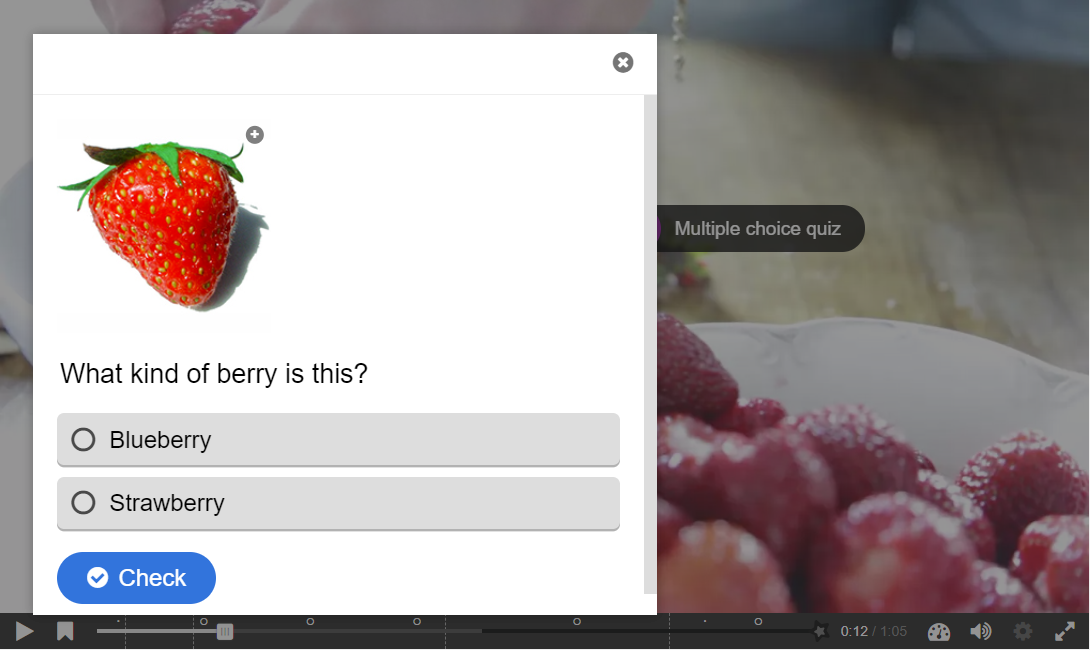
\includegraphics[width=\textwidth,center]{H5P.png}
\caption{\label{fig:H5P} Auszug aus einem \textit{Interactive Video} \citep{h5p2013video}}
\end{figure}

%%%%%%%%%%
\subsubsection{Popcorn.js}
Die Mozilla Corporation bietet mit \textit{Popcorn.js}\footnote{GitHub-Projekt, MIT Lizenz: https://github.com/mozilla/popcorn-js} eine Bibliothek an, welche neben einer standardisierten Steuerung von Medieninhalten aus verschiedenen Quellen auch die zeitabhängige Annotation von Inhalten mittels Plugins ermöglicht. Hier wäre also auch eine Entwicklung eines Plugins denkbar, mit welchem Hyperaudio-Dokumente wie gewünscht wiedergegeben werden können. Die Wartung für die Bibliothek wurde seitens Mozilla zwar eingestellt, das Projekt steht aber weiterhin auf GitHub zur Verfügung. Obwohl das Projekt nicht mehr weiterentwickelt wird, kann es durch die vorhandenen Steuerungsmöglichkeiten und das Plugin-System ein geeignetes Grundgerüst für die Entwicklung des Moodle-Plugins darstellen.

 
%%%%%%%%%%
\subsubsection{wavesurfer.js}
\label{sec:wavesurfer.js}
Bei \textit{wavesurfer.js}\footnote{GitHub-Projekt, BSD-3-Clause: https://wavesurfer-js.org; https://github.com/katspaugh/wavesurfer.js} handelt es sich um ein JavaScript-Framework, welches es ermöglicht, die Wellenform zu der abgespielten Audio-Datei visualisieren zu lassen (siehe Abbildung \ref{fig:Wavesurfer}). Diese Basisfunktionalität wurde durch Weiterentwicklungen um nützliche Funktionen erweitert. Auf zwei dieser Weiterentwicklungen wird im Folgenden eingegangen.

\begin{figure}[h!]
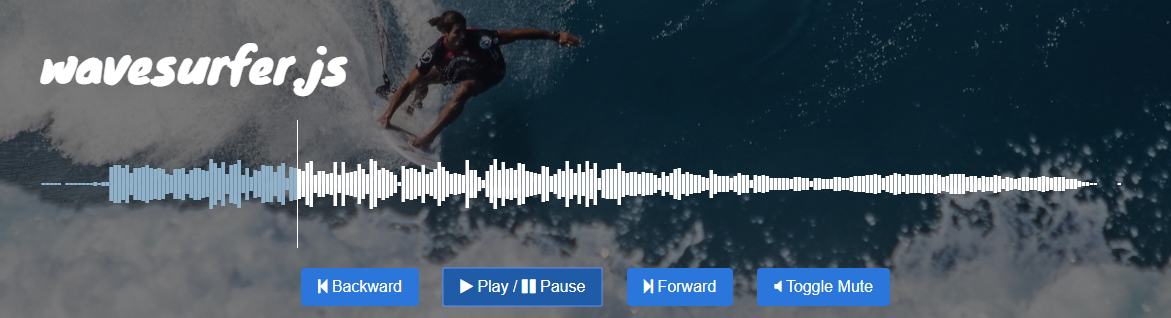
\includegraphics[width=\textwidth,center]{Wavesurfer.png}
\caption{\label{fig:Wavesurfer} Der Audio-Player auf der \textit{wavesurfer.js}-Webseite\citep{wavesurfer}}
\end{figure}


Der \textit{audio-annotator}\footnote{GitHub-Projekt, BSD-2-Clause: https://github.com/CrowdCurio/audio-annotator} stellt eine auf dem \textit{wavesurfer.js}-Framework basierende Weiterentwicklung dar, welche es mittels Weboberfläche ermöglicht, Annotationen in Form von Text an eine Audio-Datei anzuheften. Es erweitert \textit{wavesurfer.js} also um die Möglichkeit, Annotationen an eine Datei anzuheften und bietet gleichzeitig noch eine Oberfläche, um ebendiese Annotationen vorzunehmen.

Beim \textit{BAT - BMAT Annotation Tool}\footnote{GitHub-Projekt, GNU General Public License 3: https://wavesurfer-js.org; https://github.com/BlaiMelendezCatalan/BAT} handelt es sich um eine Entwicklung basierend auf dem im Zusammenhang von \textit{audio-annotator} erweiterten Frameworks \textit{wavesurfer.js}. Es ermöglicht, ebenso wie \textit{audio-annotator}, dem Benutzer mittels Weboberfläche Annotationen an einer Audio-Datei vorzunehmen. Somit bietet \textit{BAT} logischerweise dieselben Vorzüge wie bereits der \textit{audio-annotator}. Im Vergleich zum \textit{audio-annotator} stellt \textit{BAT} jedoch ein weiterentwickelteres Framework dar.

Das \textit{wavesurfer.js} Framework - speziell mit seinen Weiterenticklungen - bietet einige Funktionen, die für das Abspielen von Hyperaudio-Dokumenten nützlich sein könnten. Zusätzlich bietet es auch die Funktion,  die entsprechenden Annotationen in einer Weboberfläche an die Audio-Dateien anzuheften. Grundsätzlich lässt sich feststellen, dass \textit{wavesurfer.js} und seine Ableger im Vergleich zu den zuvor betrachteten Entwicklungen einen wesentlich unausgereifteren Eindruck hinterlassen.

%%%%%%%%%%
\subsubsection{timesheets.js}
\textit{timesheets.js}\footnote{ehemaliges GitHub-Projekt, MIT Lizenz: http://wam.inrialpes.fr/timesheets} ist ebenfalls ein JavaScript-Framemwork, welches analog zu \textit{audio-annotator} und \textit{BAT} die Annotation zusätzlicher Inhalte ermöglicht. Leider befindet sich das Framework aktuell nicht mehr in der Entwicklung. Aufgrund der Ähnlichkeit zu den {wavesurfer.js}-Ablegern und der eingestellten Entwicklung können hier zwar Ideen übernommen werden, als Basis für das zu entwickelnde Moodle-Plugin ist dieses Framework jedoch nicht geeignet.
\\\\\\
Zusammenfassend ist festzustellen, dass für die Entwicklung des Plugins für Hyperaudio-Dokumente vor allem \textit{VideoJS Player}, \textit{H5P} und \textit{Popcorn.js} die vielversprechendsten bestehenden Entwicklungen darstellen, da diese bereits einen hohen Entwicklungsstand haben. Unter Anbetracht der benötigten Funktionen stellen aber speziell der \textit{VideoJS Player} und \textit{Popcorn.js} eine gute Basis dar, da diese mit ihrem Kernelement als Player und durch die integrierten Plugin-Systeme für die Entwicklung von Multimedia-Elementen ausgelegt sind. Bei \textit{H5P} müsste die Playerfunktion mit der dazugehörigen Erweiterung für Hyperaudio-Dokumente von Grund auf entwickelt werden, um eine entsprechende interaktive Komponente für Hyperaudio-Dokumente bereitstellen zu können. Letztlich scheint \textit{Popcorn.js} die beste Grundlage für die Entwicklung des Plugins darzustellen, da hier auch die Steuerung der Medieninhalte bereits von Grund auf ausgeprägt implementiert sind, woraus bei der Umsetzung einiger Funktionen großer Nutzen gezogen werden kann. Des Weiteren ist \textit{Popcorn.js} als JavaScript-Bibliothek mühelos als Thirdparty-Framework in Moodle integrierbar.




%%%%%%%%%%
\section{Zusammenfassung}
Nachdem die Zielgruppe mittels \textit{Personas} und den dazugehörigen \textit{User Stories} definiert wurde, dienten diese der Anforderungsdefinition. Diese Anforderungen wurden dann in Hinblick auf die Zielsetzung der Arbeit in drei Prioritätsstufen eingeordnet. Anschließend wurden anhand der genaueren Betrachtung der Möglichkeiten zur Entwicklung von Plugins in Moodle die Randbedingungen bestimmt. Hierbei wurde festgehalten, dass das Plugin als Aktivitäten Plugin umzusetzen ist und dass Übersichten und Favoritenfunktion innerhalb von Blocken umgesetzte werden könnten. Mit diesem Wissen im Hinterkopf wurde dann der aktuelle Stand der Technik im allgemeinen und im Bezug auf die Entwicklung des Plugins betrachtet. In diesem Zuge wurde entschieden, dass \textit{Popcorn.js} als gute Grundlage für die Entwicklung des Plugins dient, da dieses mit seinen vorhanden Steuerungsmöglichkeiten ein gutes Grundgerüst darstellt und problemlos in Moodle integriert werden kann.

\todo[inline]{Zusammenfassung überarbeiten - mehr Ergebnisse, z.B. Anforderungen für Rollen}
